%==============================================================================
% PART 3: VQVAE ACTION TOKENIZER
%==============================================================================

\section{VQVAE Action Tokenizer}

%------------------------------------------------------------------------------
\begin{frame}{VQVAE Overview}
    \begin{block}{Purpose}
        Convert \textbf{continuous actions} to \textbf{discrete tokens} for autoregressive VLA
    \end{block}

    \vspace{0.5cm}
    \textbf{Why Tokenize Actions?}
    \begin{itemize}
        \item Leverage VLM's discrete token prediction capability
        \item Enable autoregressive generation (like text)
        \item Unified interface with language tokens
    \end{itemize}

    \vspace{0.5cm}
    \begin{alertblock}{Key Innovation}
        RDT2 uses \textbf{Residual VQ} with component separation:
        \begin{itemize}
            \item Only 27 tokens for 0.8s action chunk
            \item 3--8$\times$ shorter than prior methods
        \end{itemize}
    \end{alertblock}
\end{frame}

%------------------------------------------------------------------------------
\begin{frame}{Vector Quantization: Core Concept}
    \begin{block}{Definition}
        Map continuous encoder output $\vect{z}_e$ to nearest codebook entry $\vect{w}_k$
    \end{block}

    \vspace{0.3cm}
    \textbf{Codebook:} $\mathcal{W} = \{\vect{w}_1, \vect{w}_2, \ldots, \vect{w}_Z\}$, where $Z = 1024$

    \vspace{0.5cm}
    \textbf{Quantization:}
    \[
        k^* = \argmin_{k \in \{1, \ldots, Z\}} \| \bar{\vect{z}}_e - \bar{\vect{w}}_k \|^2
    \]

    where $\bar{\vect{z}} = \frac{\vect{z}}{\|\vect{z}\|}$ (L2 normalization)

    \vspace{0.5cm}
    \textbf{Quantized output:}
    \[
        \vect{z}_q = \vect{w}_{k^*}
    \]
\end{frame}

%------------------------------------------------------------------------------
\begin{frame}{Distance Calculation}
    \textbf{Euclidean distance with L2-normalized vectors:}

    \vspace{0.3cm}
    \[
        d(\bar{\vect{z}}_e, \bar{\vect{w}}_k) = \|\bar{\vect{z}}_e\|^2 - 2 \bar{\vect{z}}_e^T \bar{\vect{w}}_k + \|\bar{\vect{w}}_k\|^2
    \]

    \vspace{0.3cm}
    Since $\|\bar{\vect{z}}\| = 1$ after normalization:
    \[
        d(\bar{\vect{z}}_e, \bar{\vect{w}}_k) = 2 - 2 \bar{\vect{z}}_e^T \bar{\vect{w}}_k = 2(1 - \cos\theta)
    \]

    \vspace{0.5cm}
    \begin{alertblock}{Cosine Similarity}
        L2 normalization converts Euclidean distance to \textbf{cosine similarity}:
        \[
            \argmin_k d(\bar{\vect{z}}_e, \bar{\vect{w}}_k) = \argmax_k \cos(\bar{\vect{z}}_e, \bar{\vect{w}}_k)
        \]
        This improves training stability (ViT-VQGAN)
    \end{alertblock}
\end{frame}

%------------------------------------------------------------------------------
\begin{frame}{VQ Loss Functions (1/2)}
    \textbf{Three loss components:}

    \vspace{0.5cm}
    \textbf{1. Commitment Loss} (encoder $\rightarrow$ codebook):
    \[
        \mathcal{L}_{\text{commit}} = \| \vect{z}_e - \text{sg}[\vect{z}_q] \|^2
    \]

    \vspace{0.3cm}
    \textbf{2. Codebook Loss} (codebook $\rightarrow$ encoder):
    \[
        \mathcal{L}_{\text{cb}} = \| \vect{z}_q - \text{sg}[\vect{z}_e] \|^2
    \]

    \vspace{0.3cm}
    where $\text{sg}[\cdot]$ = stop-gradient operator
\end{frame}

%------------------------------------------------------------------------------
\begin{frame}{VQ Loss Functions (2/2)}
    \textbf{3. Total VQ Loss:}
    \[
        \boxed{\mathcal{L}_{\text{VQ}} = \beta \cdot \mathcal{L}_{\text{commit}} + \gamma \cdot \mathcal{L}_{\text{cb}}}
    \]

    \vspace{0.5cm}
    \begin{block}{Default Values}
        $\beta = 0.25$ (commitment\_cost), $\gamma = 0$ (codebook\_cost)
    \end{block}

    \vspace{0.3cm}
    \begin{alertblock}{Note}
        With EMA codebook updates, $\gamma = 0$ is typical since the codebook is updated directly via exponential moving average rather than gradient descent.
    \end{alertblock}
\end{frame}

%------------------------------------------------------------------------------
\begin{frame}{Straight-Through Estimator}
    \begin{columns}[T]
        \begin{column}{0.5\textwidth}
            \begin{block}{Problem}
                Quantization is \textbf{non-differentiable}
            \end{block}

            \vspace{0.2cm}
            \textbf{Forward pass:}
            \[
                \vect{z}_q = \text{Quantize}(\vect{z}_e) = \vect{w}_{k^*}
            \]

            \textbf{Backward pass:}
            \[
                \frac{\partial \mathcal{L}}{\partial \vect{z}_e} = \frac{\partial \mathcal{L}}{\partial \vect{z}_q}
            \]
        \end{column}
        \begin{column}{0.5\textwidth}
            \textbf{Implementation:}
            \[
                \boxed{\vect{z}_q = \vect{z}_e + \text{sg}[\vect{z}_q - \vect{z}_e]}
            \]

            \vspace{0.3cm}
            \begin{alertblock}{Interpretation}
                Forward: output is $\vect{z}_q$ \\
                Backward: gradient $\to \vect{z}_e$
            \end{alertblock}
        \end{column}
    \end{columns}
\end{frame}

%------------------------------------------------------------------------------
\begin{frame}{EMA Codebook Update}
    \begin{columns}[T]
        \begin{column}{0.55\textwidth}
            \textbf{Track cluster statistics:}
            \begin{itemize}
                \item $N_i^{(t)}$: count for entry $i$
                \item $\vect{m}_i^{(t)}$: sum of assigned vectors
            \end{itemize}

            \vspace{0.2cm}
            \textbf{EMA Update Rules:}
            \begin{align*}
                N_i^{(t)} &= \gamma N_i^{(t-1)} + (1 - \gamma) n_i \\
                \vect{m}_i^{(t)} &= \gamma \vect{m}_i^{(t-1)} + (1 - \gamma) \textstyle\sum_j \vect{z}_e^{(j)}
            \end{align*}
        \end{column}
        \begin{column}{0.45\textwidth}
            \textbf{Codebook Update:}
            \[
                \boxed{\vect{w}_i = \frac{\vect{m}_i}{\tilde{N}_i}}
            \]

            \textbf{Laplace smoothing:}
            \[
                \tilde{N}_i = \frac{N_i + \epsilon}{N + Z\epsilon} N
            \]

            \vspace{0.2cm}
            Default: $\gamma = 0.99$, $\epsilon = 10^{-5}$
        \end{column}
    \end{columns}
\end{frame}

%------------------------------------------------------------------------------
\begin{frame}{Factorized Codes}
    \begin{block}{Motivation}
        Improve codebook utilization by separating dimensions
    \end{block}

    \vspace{0.3cm}
    \textbf{Architecture:}
    \begin{center}
    \begin{tikzpicture}[
        box/.style={rectangle, draw, minimum width=1.5cm, minimum height=0.7cm, align=center, font=\small},
        arrow/.style={->, thick},
        scale=0.85, transform shape
    ]
        \node[box, fill=encoderblue!30] (ze) at (0,0) {$\vect{z}_e$\\{\tiny latent}};
        \node[box, fill=vqpurple!30] (proj_in) at (2.5,0) {in\_proj};
        \node[box, fill=codebookpink!30] (vq) at (5,0) {VQ};
        \node[box, fill=vqpurple!30] (proj_out) at (7.5,0) {out\_proj};
        \node[box, fill=decodergreen!30] (zq) at (10,0) {$\vect{z}_q$\\{\tiny latent}};

        \draw[arrow] (ze) -- (proj_in);
        \draw[arrow] (proj_in) -- (vq);
        \draw[arrow] (vq) -- (proj_out);
        \draw[arrow] (proj_out) -- (zq);
    \end{tikzpicture}
    \end{center}

    \vspace{0.3cm}
    \textbf{Dimension Flow:}
    \[
        64 \xrightarrow{\text{in\_proj}} 256 \xrightarrow{\text{VQ}} 256 \xrightarrow{\text{out\_proj}} 64
    \]

    \begin{alertblock}{Benefit}
        Codebook lookup in lower-dimensional space improves usage
    \end{alertblock}
\end{frame}

%------------------------------------------------------------------------------
\begin{frame}{Codebook Restart (1/2)}
    \begin{block}{Problem: Dead Entries}
        Some codebook entries are never selected $\rightarrow$ wasted capacity
    \end{block}

    \vspace{0.5cm}
    \textbf{Tracking Dead Entries:}
    \begin{itemize}
        \item Maintain \code{entry\_hits} buffer of size $[P, Z]$
        \item $P = 64$ (restart period), $Z = 1024$ (codebook size)
        \item Track which entries were selected each iteration
    \end{itemize}

    \vspace{0.3cm}
    \textbf{Restart Condition (every $P$ iterations):}
    \[
        \text{dead\_entries} = \{ i : \sum_{t=1}^{P} \text{hits}_{t,i} = 0 \}
    \]
\end{frame}

%------------------------------------------------------------------------------
\begin{frame}{Codebook Restart (2/2)}
    \textbf{Restart Process:}
    \begin{enumerate}
        \item Gather encoder outputs from all GPUs
        \item Randomly select from current batch
        \item Re-initialize dead entries with selected vectors
    \end{enumerate}

    \vspace{0.5cm}
    \begin{alertblock}{Implementation Detail}
        \begin{itemize}
            \item Uses \code{dist.all\_gather} for multi-GPU synchronization
            \item Random sampling ensures diversity
            \item Effectively performs online k-means update
        \end{itemize}
    \end{alertblock}
\end{frame}

%------------------------------------------------------------------------------
\begin{frame}{Residual VQ Algorithm}
    \begin{columns}[T]
        \begin{column}{0.55\textwidth}
            \begin{block}{Key Idea}
                Quantize residuals iteratively
            \end{block}

            \vspace{0.2cm}
            \textbf{Algorithm:}
            \begin{algorithmic}[1]
                \State $\vect{r} \leftarrow \vect{z}$, $\vect{z}_q \leftarrow \vect{0}$
                \For{$i = 1$ to $N$}
                    \State $\vect{z}_{q,i}, idx_i \leftarrow VQ_i(\vect{r})$
                    \State $\vect{z}_q \leftarrow \vect{z}_q + \vect{z}_{q,i}$
                    \State $\vect{r} \leftarrow \vect{r} - \vect{z}_{q,i}$
                \EndFor
                \State \textbf{Return:} $\vect{z}_q$, $[idx_1, \ldots, idx_N]$
            \end{algorithmic}
        \end{column}
        \begin{column}{0.4\textwidth}
            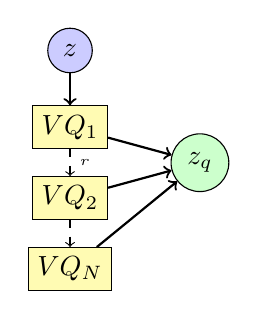
\begin{tikzpicture}[scale=0.75]
                \node[draw, circle, fill=blue!20] (z) at (0,2.5) {$\vect{z}$};
                \node[draw, rectangle, fill=yellow!30] (vq1) at (0,1.2) {$VQ_1$};
                \node[draw, rectangle, fill=yellow!30] (vq2) at (0,0) {$VQ_2$};
                \node[draw, rectangle, fill=yellow!30] (vq3) at (0,-1.2) {$VQ_N$};
                \node[draw, circle, fill=green!20] (zq) at (2.2,0.6) {$\vect{z}_q$};

                \draw[->, thick] (z) -- (vq1);
                \draw[->, dashed] (vq1) -- node[right, font=\tiny] {$\vect{r}$} (vq2);
                \draw[->, dashed] (vq2) -- (vq3);
                \draw[->, thick] (vq1) -- (zq);
                \draw[->, thick] (vq2) -- (zq);
                \draw[->, thick] (vq3) -- (zq);
            \end{tikzpicture}

            \vspace{0.2cm}
            \textbf{Decoding:}
            \[
                \vect{z}_q = \textstyle\sum_i VQ_i(idx_i)
            \]
        \end{column}
    \end{columns}
\end{frame}

%------------------------------------------------------------------------------
\begin{frame}{Residual VQ: Visual Process}
    \begin{center}
    \begin{tikzpicture}[
        box/.style={rectangle, draw, rounded corners, minimum width=1.4cm, minimum height=0.6cm, align=center, font=\scriptsize},
        arrow/.style={->, thick, >=stealth},
        scale=0.75, transform shape
    ]
        % Main horizontal flow - residuals
        \node[box, fill=blue!20] (input) at (0,0) {Input $\mathbf{z}$};
        \node[box, fill=yellow!30] (r1) at (4,0) {$\mathbf{r}_1$};
        \node[box, fill=yellow!30] (r2) at (8,0) {$\mathbf{r}_2$};
        \node[box, fill=gray!20] (r3) at (12,0) {$\mathbf{r}_3 \approx 0$};

        % Codebooks above
        \node[box, fill=codebookpink] (cb1) at (2,1.8) {Codebook 1};
        \node[box, fill=codebookpink] (cb2) at (6,1.8) {Codebook 2};
        \node[box, fill=codebookpink] (cb3) at (10,1.8) {Codebook 3};

        % Quantized values below codebooks
        \node[box, fill=vqpurple!30] (q1) at (2,3.5) {$\hat{\mathbf{z}}_1$};
        \node[box, fill=vqpurple!30] (q2) at (6,3.5) {$\hat{\mathbf{z}}_2$};
        \node[box, fill=vqpurple!30] (q3) at (10,3.5) {$\hat{\mathbf{z}}_3$};

        % Final output
        \node[box, fill=rdtgreen!30] (output) at (13,3.5) {$\sum_i \hat{\mathbf{z}}_i$};

        % Arrows - main flow (input to residuals via codebooks)
        \draw[arrow] (input) -- (cb1);
        \draw[arrow] (cb1) -- (q1);
        \draw[arrow] (cb1) -- (r1);

        \draw[arrow] (r1) -- (cb2);
        \draw[arrow] (cb2) -- (q2);
        \draw[arrow] (cb2) -- (r2);

        \draw[arrow] (r2) -- (cb3);
        \draw[arrow] (cb3) -- (q3);
        \draw[arrow] (cb3) -- (r3);

        % Arrows - quantized to sum (horizontal at top)
        \draw[arrow] (q1) -- (q2);
        \draw[arrow] (q2) -- (q3);
        \draw[arrow] (q3) -- (output);

        % Label for sum path
        \node[font=\tiny, above] at (4,3.5) {+};
        \node[font=\tiny, above] at (8,3.5) {+};

        % Residual magnitude bar chart
        \begin{scope}[shift={(0,-2.5)}]
            \draw[->] (0,0) -- (11,0) node[right, font=\scriptsize] {Stage};
            \draw[->] (0,0) -- (0,1.3) node[above, font=\scriptsize] {$\|\mathbf{r}\|$};
            \fill[blue!40] (1,0) rectangle (2.2,1.0);
            \fill[blue!40] (4,0) rectangle (5.2,0.5);
            \fill[blue!40] (7,0) rectangle (8.2,0.25);
            \fill[blue!40] (10,0) rectangle (11.2,0.08);
            \node[font=\tiny] at (1.6,-0.25) {Input};
            \node[font=\tiny] at (4.6,-0.25) {After 1};
            \node[font=\tiny] at (7.6,-0.25) {After 2};
            \node[font=\tiny] at (10.6,-0.25) {After 3};
        \end{scope}
    \end{tikzpicture}
    \end{center}
\end{frame}

%------------------------------------------------------------------------------
\begin{frame}{RVQ: Mathematical Formulation}
    \begin{columns}[T]
        \begin{column}{0.5\textwidth}
            \textbf{Encoding (per timestep):}
            \begin{align*}
                \vect{r}^{(0)} &= \vect{z} \\
                \vect{z}_{q}^{(i)}, idx^{(i)} &= VQ_i(\vect{r}^{(i-1)}) \\
                \vect{r}^{(i)} &= \vect{r}^{(i-1)} - \vect{z}_{q}^{(i)}
            \end{align*}

            \textbf{Final Output:}
            \[
                \boxed{\vect{z}_q = \sum_{i=1}^{N} \vect{z}_{q}^{(i)}}
            \]
        \end{column}
        \begin{column}{0.5\textwidth}
            \textbf{Loss Aggregation:}
            \[
                \mathcal{L}_{\text{RVQ}} = \sum_{i=1}^{N} \mathcal{L}_{\text{VQ}}^{(i)}
            \]

            \vspace{0.3cm}
            \begin{block}{Token Sequence}
                $N$ codebooks $\rightarrow$ $N$ tokens/timestep \\
                Each token $\in \{0, \ldots, 1023\}$
            \end{block}
        \end{column}
    \end{columns}
\end{frame}

%------------------------------------------------------------------------------
\begin{frame}{Encoder CNN Architecture}
    \textbf{8$\times$ Temporal Compression:} $[B, D, 24] \rightarrow [B, C, 3]$

    \vspace{0.3cm}
    \begin{center}
    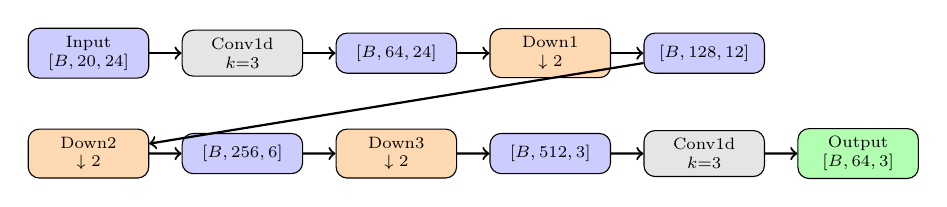
\begin{tikzpicture}[
        block/.style={rectangle, draw, rounded corners, minimum width=1.8cm, minimum height=0.6cm, align=center, font=\scriptsize},
        arrow/.style={->, thick},
        scale=0.85, transform shape
    ]
        % Input
        \node[block, fill=blue!20] (input) at (0,0) {Input\\$[B, 20, 24]$};

        % Conv in
        \node[block, fill=gray!20] (conv_in) at (2.3,0) {Conv1d\\$k{=}3$};
        \node[block, fill=blue!20] (c1) at (4.6,0) {$[B, 64, 24]$};

        % Down block 1
        \node[block, fill=orange!30] (down1) at (6.9,0) {Down1\\$\downarrow 2$};
        \node[block, fill=blue!20] (c2) at (9.2,0) {$[B, 128, 12]$};

        % Down block 2
        \node[block, fill=orange!30] (down2) at (0,-1.5) {Down2\\$\downarrow 2$};
        \node[block, fill=blue!20] (c3) at (2.3,-1.5) {$[B, 256, 6]$};

        % Down block 3
        \node[block, fill=orange!30] (down3) at (4.6,-1.5) {Down3\\$\downarrow 2$};
        \node[block, fill=blue!20] (c4) at (6.9,-1.5) {$[B, 512, 3]$};

        % Conv out
        \node[block, fill=gray!20] (conv_out) at (9.2,-1.5) {Conv1d\\$k{=}3$};
        \node[block, fill=green!30] (output) at (11.5,-1.5) {Output\\$[B, 64, 3]$};

        \draw[arrow] (input) -- (conv_in);
        \draw[arrow] (conv_in) -- (c1);
        \draw[arrow] (c1) -- (down1);
        \draw[arrow] (down1) -- (c2);
        \draw[arrow] (c2) -- (down2);
        \draw[arrow] (down2) -- (c3);
        \draw[arrow] (c3) -- (down3);
        \draw[arrow] (down3) -- (c4);
        \draw[arrow] (c4) -- (conv_out);
        \draw[arrow] (conv_out) -- (output);
    \end{tikzpicture}
    \end{center}

    \vspace{0.3cm}
    \textbf{Down Block Structure:}
    \[
        \text{ConvBlock}(ch \rightarrow 2ch) \rightarrow \text{Downsample2x} \rightarrow \text{ConvBlock}
    \]

    \textbf{ConvBlock:} GroupNorm $\rightarrow$ SiLU $\rightarrow$ Conv1d $\rightarrow$ Dropout
\end{frame}

%------------------------------------------------------------------------------
\begin{frame}{Decoder CNN Architecture}
    \textbf{8$\times$ Temporal Upsampling:} $[B, C, 3] \rightarrow [B, D, 24]$

    \vspace{0.3cm}
    \begin{center}
    \begin{tikzpicture}[
        block/.style={rectangle, draw, rounded corners, minimum width=1.8cm, minimum height=0.6cm, align=center, font=\scriptsize},
        arrow/.style={->, thick},
        scale=0.85, transform shape
    ]
        % Input
        \node[block, fill=green!30] (input) at (0,0) {Input\\$[B, 64, 3]$};

        % Conv in
        \node[block, fill=gray!20] (conv_in) at (2.3,0) {Conv1d\\$k{=}3$};
        \node[block, fill=blue!20] (c1) at (4.6,0) {$[B, 512, 3]$};

        % Up block 1
        \node[block, fill=rdtgreen!30] (up1) at (6.9,0) {Up1\\$\uparrow 2$};
        \node[block, fill=blue!20] (c2) at (9.2,0) {$[B, 256, 6]$};

        % Up block 2
        \node[block, fill=rdtgreen!30] (up2) at (0,-1.5) {Up2\\$\uparrow 2$};
        \node[block, fill=blue!20] (c3) at (2.3,-1.5) {$[B, 128, 12]$};

        % Up block 3
        \node[block, fill=rdtgreen!30] (up3) at (4.6,-1.5) {Up3\\$\uparrow 2$};
        \node[block, fill=blue!20] (c4) at (6.9,-1.5) {$[B, 64, 24]$};

        % Conv out
        \node[block, fill=gray!20] (conv_out) at (9.2,-1.5) {Conv1d\\$k{=}3$};
        \node[block, fill=blue!20] (output) at (11.5,-1.5) {Output\\$[B, 20, 24]$};

        \draw[arrow] (input) -- (conv_in);
        \draw[arrow] (conv_in) -- (c1);
        \draw[arrow] (c1) -- (up1);
        \draw[arrow] (up1) -- (c2);
        \draw[arrow] (c2) -- (up2);
        \draw[arrow] (up2) -- (c3);
        \draw[arrow] (c3) -- (up3);
        \draw[arrow] (up3) -- (c4);
        \draw[arrow] (c4) -- (conv_out);
        \draw[arrow] (conv_out) -- (output);
    \end{tikzpicture}
    \end{center}

    \vspace{0.3cm}
    \textbf{Up Block Structure:}
    \[
        \text{ConvBlock} \rightarrow \text{Upsample2x\_TF} \rightarrow \text{ConvBlock}(ch \rightarrow ch/2)
    \]

    \textbf{Upsample2x\_TF:} Transposed convolution with $k=4$, $s=2$, $p=1$
\end{frame}

%------------------------------------------------------------------------------
\begin{frame}{MultiVQVAE: Component Separation}
    \begin{block}{Key Innovation}
        Separate tokenizers for \textbf{position}, \textbf{rotation}, and \textbf{gripper}
    \end{block}

    \vspace{0.3cm}
    \begin{center}
    \begin{tikzpicture}[
        box/.style={rectangle, draw, rounded corners, minimum width=2.2cm, minimum height=0.8cm, align=center, font=\small},
        arrow/.style={->, thick},
        scale=0.85, transform shape
    ]
        % Input
        \node[box, fill=blue!20] (input) at (0,0) {Action\\$[B, 24, 20]$};

        % Split
        \node[box, fill=encoderblue!30] (pos) at (3.5,1.2) {Position\\$[B, 24, 6]$};
        \node[box, fill=vqpurple!30] (rot) at (3.5,0) {Rotation\\$[B, 24, 12]$};
        \node[box, fill=actionorange!30] (grip) at (3.5,-1.2) {Gripper\\$[B, 24, 2]$};

        % VQVAEs
        \node[box, fill=yellow!30] (vq_pos) at (7,1.2) {VQVAE$_\text{pos}$\\6 codebooks};
        \node[box, fill=yellow!30] (vq_rot) at (7,0) {VQVAE$_\text{rot}$\\3 codebooks};
        \node[box, fill=yellow!30] (vq_grip) at (7,-1.2) {VQVAE$_\text{grip}$\\1 codebook};

        % Tokens
        \node[box, fill=green!30] (tok_pos) at (10.5,1.2) {18 tokens};
        \node[box, fill=green!30] (tok_rot) at (10.5,0) {9 tokens};
        \node[box, fill=green!30] (tok_grip) at (10.5,-1.2) {3 tokens};

        \draw[arrow] (input) -- (pos);
        \draw[arrow] (input) -- (rot);
        \draw[arrow] (input) -- (grip);
        \draw[arrow] (pos) -- (vq_pos);
        \draw[arrow] (rot) -- (vq_rot);
        \draw[arrow] (grip) -- (vq_grip);
        \draw[arrow] (vq_pos) -- (tok_pos);
        \draw[arrow] (vq_rot) -- (tok_rot);
        \draw[arrow] (vq_grip) -- (tok_grip);
    \end{tikzpicture}
    \end{center}

    \vspace{0.3cm}
    \textbf{Total Tokens:} $18 + 9 + 3 = 30 \rightarrow 27$ (after optimization)
\end{frame}

%------------------------------------------------------------------------------
\begin{frame}{Token Distribution}
    \begin{table}
        \centering
        \renewcommand{\arraystretch}{1.4}
        \begin{tabular}{lcccc}
            \toprule
            \textbf{Component} & \textbf{Dim} & \textbf{Codebooks} & \textbf{Timesteps} & \textbf{Tokens} \\
            \midrule
            Position & 6 & 6 & 3 & $6 \times 3 = 18$ \\
            Rotation & 12 & 3 & 3 & $3 \times 3 = 9$ \\
            Gripper & 2 & 1 & 3 & $1 \times 3 = 3$ \\
            \midrule
            \textbf{Total} & 20 & 10 & -- & \textbf{30 $\rightarrow$ 27} \\
            \bottomrule
        \end{tabular}
    \end{table}

    \vspace{0.5cm}
    \textbf{Compression Analysis:}
    \begin{itemize}
        \item Input: $24 \times 20 = 480$ float values
        \item Output: 27 discrete tokens
        \item Compression ratio: $\sim$18$\times$
        \item Each token: $\log_2(1024) = 10$ bits
    \end{itemize}
\end{frame}

%------------------------------------------------------------------------------
\begin{frame}{Action Dimension Mapping}
    \begin{columns}[T]
        \begin{column}{0.5\textwidth}
            \textbf{20-dim $\rightarrow$ 3 Components:}
            \begin{table}
                \centering
                \renewcommand{\arraystretch}{1.2}
                \footnotesize
                \begin{tabular}{lcc}
                    \toprule
                    & \textbf{Right} & \textbf{Left} \\
                    \midrule
                    Position & [0:3] & [10:13] \\
                    Rotation & [3:9] & [13:19] \\
                    Gripper & [9] & [19] \\
                    \bottomrule
                \end{tabular}
            \end{table}
        \end{column}
        \begin{column}{0.5\textwidth}
            \textbf{Code Implementation:}
            \begin{itemize}
                \item \code{select\_act\_dim(x, 'pos')}
                \item \code{select\_act\_dim(x, 'rot')}
                \item \code{select\_act\_dim(x, 'grip')}
            \end{itemize}

            \vspace{0.2cm}
            \textbf{Reconstruction:}
            \begin{itemize}
                \item \code{apply\_act\_dim(x, y, type)}
            \end{itemize}
        \end{column}
    \end{columns}
\end{frame}

%------------------------------------------------------------------------------
\begin{frame}{Token Conversion: VLA $\leftrightarrow$ VAE}
    \begin{columns}[T]
        \begin{column}{0.5\textwidth}
            \begin{block}{Problem}
                VLA tokens $\neq$ VAE indices
            \end{block}

            \vspace{0.3cm}
            \textbf{VLA to VAE:}
            \[
                \boxed{t_{\text{vae}} = V - (t_{\text{vla}} + 1)}
            \]

            \textbf{VAE to VLA:}
            \[
                \boxed{t_{\text{vla}} = V - t_{\text{vae}} - 1}
            \]

            {\small $V = 152064$ (vocab size)}
        \end{column}
        \begin{column}{0.5\textwidth}
            \textbf{Clamping:}
            \[
                t_{\text{vae}} = \text{clamp}(t_{\text{vae}}, 0, 1023)
            \]

            \vspace{0.3cm}
            \begin{alertblock}{Note}
                Invalid tokens indicate generation errors
            \end{alertblock}
        \end{column}
    \end{columns}
\end{frame}

%------------------------------------------------------------------------------
\begin{frame}{Complete VQVAE Pipeline}
    \begin{center}
    \begin{tikzpicture}[
        box/.style={rectangle, draw, rounded corners, minimum width=1.8cm, minimum height=0.7cm, align=center, font=\scriptsize},
        arrow/.style={->, thick},
        scale=0.85, transform shape
    ]
        % Encoding path
        \node[box, fill=blue!20] (input) at (0,2) {Action\\$[B,24,20]$};
        \node[box, fill=gray!30] (perm1) at (2.5,2) {permute\\$(0,2,1)$};
        \node[box, fill=encoderblue!30] (enc) at (5,2) {Encoder\\CNN};
        \node[box, fill=blue!20] (latent) at (7.5,2) {Latent\\$[B,64,3]$};
        \node[box, fill=gray!30] (reshape1) at (10,2) {reshape\\$[B{\cdot}3,64]$};
        \node[box, fill=vqpurple!30] (rvq) at (12.5,2) {RVQ};

        % Token output
        \node[box, fill=green!30] (tokens) at (12.5,0) {Tokens\\$[B,27]$};

        % Decoding path
        \node[box, fill=vqpurple!30] (rvq_dec) at (10,0) {RVQ\\decode};
        \node[box, fill=gray!30] (reshape2) at (7.5,0) {reshape\\$[B,64,3]$};
        \node[box, fill=decodergreen!30] (dec) at (5,0) {Decoder\\CNN};
        \node[box, fill=gray!30] (perm2) at (2.5,0) {permute\\$(0,2,1)$};
        \node[box, fill=blue!20] (output) at (0,0) {Recon\\$[B,24,20]$};

        % Arrows
        \draw[arrow] (input) -- (perm1);
        \draw[arrow] (perm1) -- (enc);
        \draw[arrow] (enc) -- (latent);
        \draw[arrow] (latent) -- (reshape1);
        \draw[arrow] (reshape1) -- (rvq);
        \draw[arrow] (rvq) -- (tokens);
        \draw[arrow] (tokens) -- (rvq_dec);
        \draw[arrow] (rvq_dec) -- (reshape2);
        \draw[arrow] (reshape2) -- (dec);
        \draw[arrow] (dec) -- (perm2);
        \draw[arrow] (perm2) -- (output);
    \end{tikzpicture}
    \end{center}

    \vspace{0.5cm}
    \textbf{Key Dimension Transformations:}
    \begin{align*}
        [B, 24, 20] &\xrightarrow{\text{permute}} [B, 20, 24] \xrightarrow{\text{Encoder}} [B, 64, 3] \\
        &\xrightarrow{\text{reshape}} [B \cdot 3, 64] \xrightarrow{\text{RVQ}} [B \cdot 3, N] \\
        &\xrightarrow{\text{flatten}} [B, 3 \cdot N] = [B, 27]
    \end{align*}
\end{frame}

%------------------------------------------------------------------------------
\begin{frame}{Codebook Parameters (1/2)}
    \begin{table}
        \centering
        \renewcommand{\arraystretch}{1.3}
        \begin{tabular}{lccc}
            \toprule
            \textbf{Parameter} & \textbf{Position} & \textbf{Rotation} & \textbf{Gripper} \\
            \midrule
            Input dim ($D$) & 6 & 12 & 2 \\
            Latent dim ($C$) & 64 & 64 & 64 \\
            Embedding dim ($E$) & 256 & 256 & 256 \\
            Codebook size ($Z$) & 1024 & 1024 & 1024 \\
            Num codebooks ($N$) & 6 & 3 & 1 \\
            \bottomrule
        \end{tabular}
    \end{table}
\end{frame}

%------------------------------------------------------------------------------
\begin{frame}{Codebook Parameters (2/2)}
    \textbf{Token Output Summary:}
    \begin{table}
        \centering
        \renewcommand{\arraystretch}{1.3}
        \begin{tabular}{lccc}
            \toprule
            & \textbf{Position} & \textbf{Rotation} & \textbf{Gripper} \\
            \midrule
            Tokens per timestep & 6 & 3 & 1 \\
            Timesteps & 3 & 3 & 3 \\
            \textbf{Total tokens} & \textbf{18} & \textbf{9} & \textbf{3} \\
            \bottomrule
        \end{tabular}
    \end{table}

    \vspace{0.5cm}
    \begin{block}{Default Hyperparameters}
        \begin{itemize}
            \item EMA decay: $\gamma = 0.99$
            \item Commitment cost: $\beta = 0.25$
            \item Codebook restart interval: 64 iterations
        \end{itemize}
    \end{block}
\end{frame}

%------------------------------------------------------------------------------
\begin{frame}{VQVAE Loss Components (1/2)}
    \textbf{Total Training Loss:}
    \[
        \mathcal{L}_{\text{total}} = \mathcal{L}_{\text{recon}} + \mathcal{L}_{\text{VQ}}
    \]

    \vspace{0.3cm}
    \textbf{1. Reconstruction Loss (per component):}
    \begin{itemize}
        \item Position: MSE loss
              \[ \mathcal{L}_{\text{pos}} = \|\hat{\vect{p}} - \vect{p}\|^2 \]
        \item Rotation: Geodesic loss (6D representation)
              \[ \mathcal{L}_{\text{rot}} = \arccos\left(\frac{\text{tr}(\mat{R}_{\text{pred}}^T \mat{R}_{\text{gt}}) - 1}{2}\right) \]
    \end{itemize}
\end{frame}

%------------------------------------------------------------------------------
\begin{frame}{VQVAE Loss Components (2/2)}
    \textbf{1. Reconstruction Loss (continued):}
    \begin{itemize}
        \item Gripper: MSE loss
              \[ \mathcal{L}_{\text{grip}} = \|\hat{g} - g\|^2 \]
    \end{itemize}

    \vspace{0.5cm}
    \textbf{2. VQ Loss:}
    \[
        \mathcal{L}_{\text{VQ}} = \sum_{c \in \{\text{pos}, \text{rot}, \text{grip}\}} \mathcal{L}_{\text{VQ}}^{(c)}
    \]

    \vspace{0.3cm}
    \begin{block}{Total Loss}
        \[
            \mathcal{L}_{\text{total}} = \mathcal{L}_{\text{pos}} + \mathcal{L}_{\text{rot}} + \mathcal{L}_{\text{grip}} + \mathcal{L}_{\text{VQ}}
        \]
    \end{block}
\end{frame}

%------------------------------------------------------------------------------
\begin{frame}[fragile]{HuggingFace Model (1/2)}
    \textbf{Model Location:}
    \code{robotics-diffusion-transformer/RVQActionTokenizer}

    \vspace{0.5cm}
    \textbf{Loading in Code:}
    \begin{lstlisting}[language=Python]
from vqvae.models.multivqvae import MultiVQVAE

vae = MultiVQVAE.from_pretrained(
    "robotics-diffusion-transformer/RVQActionTokenizer"
)
vae = vae.to("cuda").float()
    \end{lstlisting}
\end{frame}

%------------------------------------------------------------------------------
\begin{frame}{HuggingFace Model (2/2)}
    \textbf{Key Attributes:}
    \begin{itemize}
        \item \code{vae.pos\_id\_len} = 18
        \item \code{vae.rot\_id\_len} = 9
        \item \code{vae.grip\_id\_len} = 3
        \item \code{vae.num\_embeddings} = 1024
    \end{itemize}
\end{frame}

%------------------------------------------------------------------------------
\begin{frame}[fragile]{Encode/Decode Example (1/2)}
    \textbf{Encoding Actions to Tokens:}
    \begin{lstlisting}[language=Python]
# actions: [B, 24, 20] - normalized action chunk
with torch.no_grad():
    tokens = vae.encode(actions)  # [B, 27]
    \end{lstlisting}

    \vspace{0.5cm}
    \textbf{Decoding Tokens to Actions:}
    \begin{lstlisting}[language=Python]
# tokens: [B, 27] - from VLA generation
with torch.no_grad():
    actions_recon = vae.decode(tokens)  # [B, 24, 20]
    \end{lstlisting}
\end{frame}

%------------------------------------------------------------------------------
\begin{frame}[fragile]{Encode/Decode Example (2/2)}
    \textbf{Component-wise Decoding:}
    \begin{lstlisting}[language=Python]
result = vae.decode(tokens, return_dict=True)
# result['pos']: [B, 24, 6]
# result['rot']: [B, 24, 12]
# result['grip']: [B, 24, 2]
    \end{lstlisting}
\end{frame}

%------------------------------------------------------------------------------
\begin{frame}{VQVAE Summary (1/2)}
    \begin{columns}[T]
        \begin{column}{0.5\textwidth}
            \textbf{Key Techniques:}
            \begin{itemize}
                \item L2 normalization (cosine similarity)
                \item Straight-through estimator
                \item EMA codebook updates
                \item Codebook restart for dead entries
                \item Residual quantization
                \item Component separation
            \end{itemize}
        \end{column}
        \begin{column}{0.5\textwidth}
            \textbf{Output Specification:}
            \begin{itemize}
                \item 27 discrete tokens
                \item Each token $\in [0, 1023]$
                \item Position: 18 tokens
                \item Rotation: 9 tokens
                \item Gripper: 3 tokens
            \end{itemize}
        \end{column}
    \end{columns}
\end{frame}

%------------------------------------------------------------------------------
\begin{frame}{VQVAE Summary (2/2)}
    \begin{alertblock}{Comparison with Prior Methods}
        \begin{itemize}
            \item ACT: 256 tokens per chunk
            \item RT-2: 256 tokens per step
            \item \textbf{RDT2: 27 tokens per chunk (0.8s)}
            \item $\mathbf{3\text{--}8\times}$ \textbf{shorter token sequences}
        \end{itemize}
    \end{alertblock}

    \vspace{0.5cm}
    \begin{block}{Key Benefits}
        \begin{itemize}
            \item Faster autoregressive generation
            \item Lower compute requirements
            \item Unified bimanual action representation
        \end{itemize}
    \end{block}
\end{frame}

